
\appendices




\section{Design}\label{sec:appendix-design}  % Felix


\begin{figure*}[!thb]
    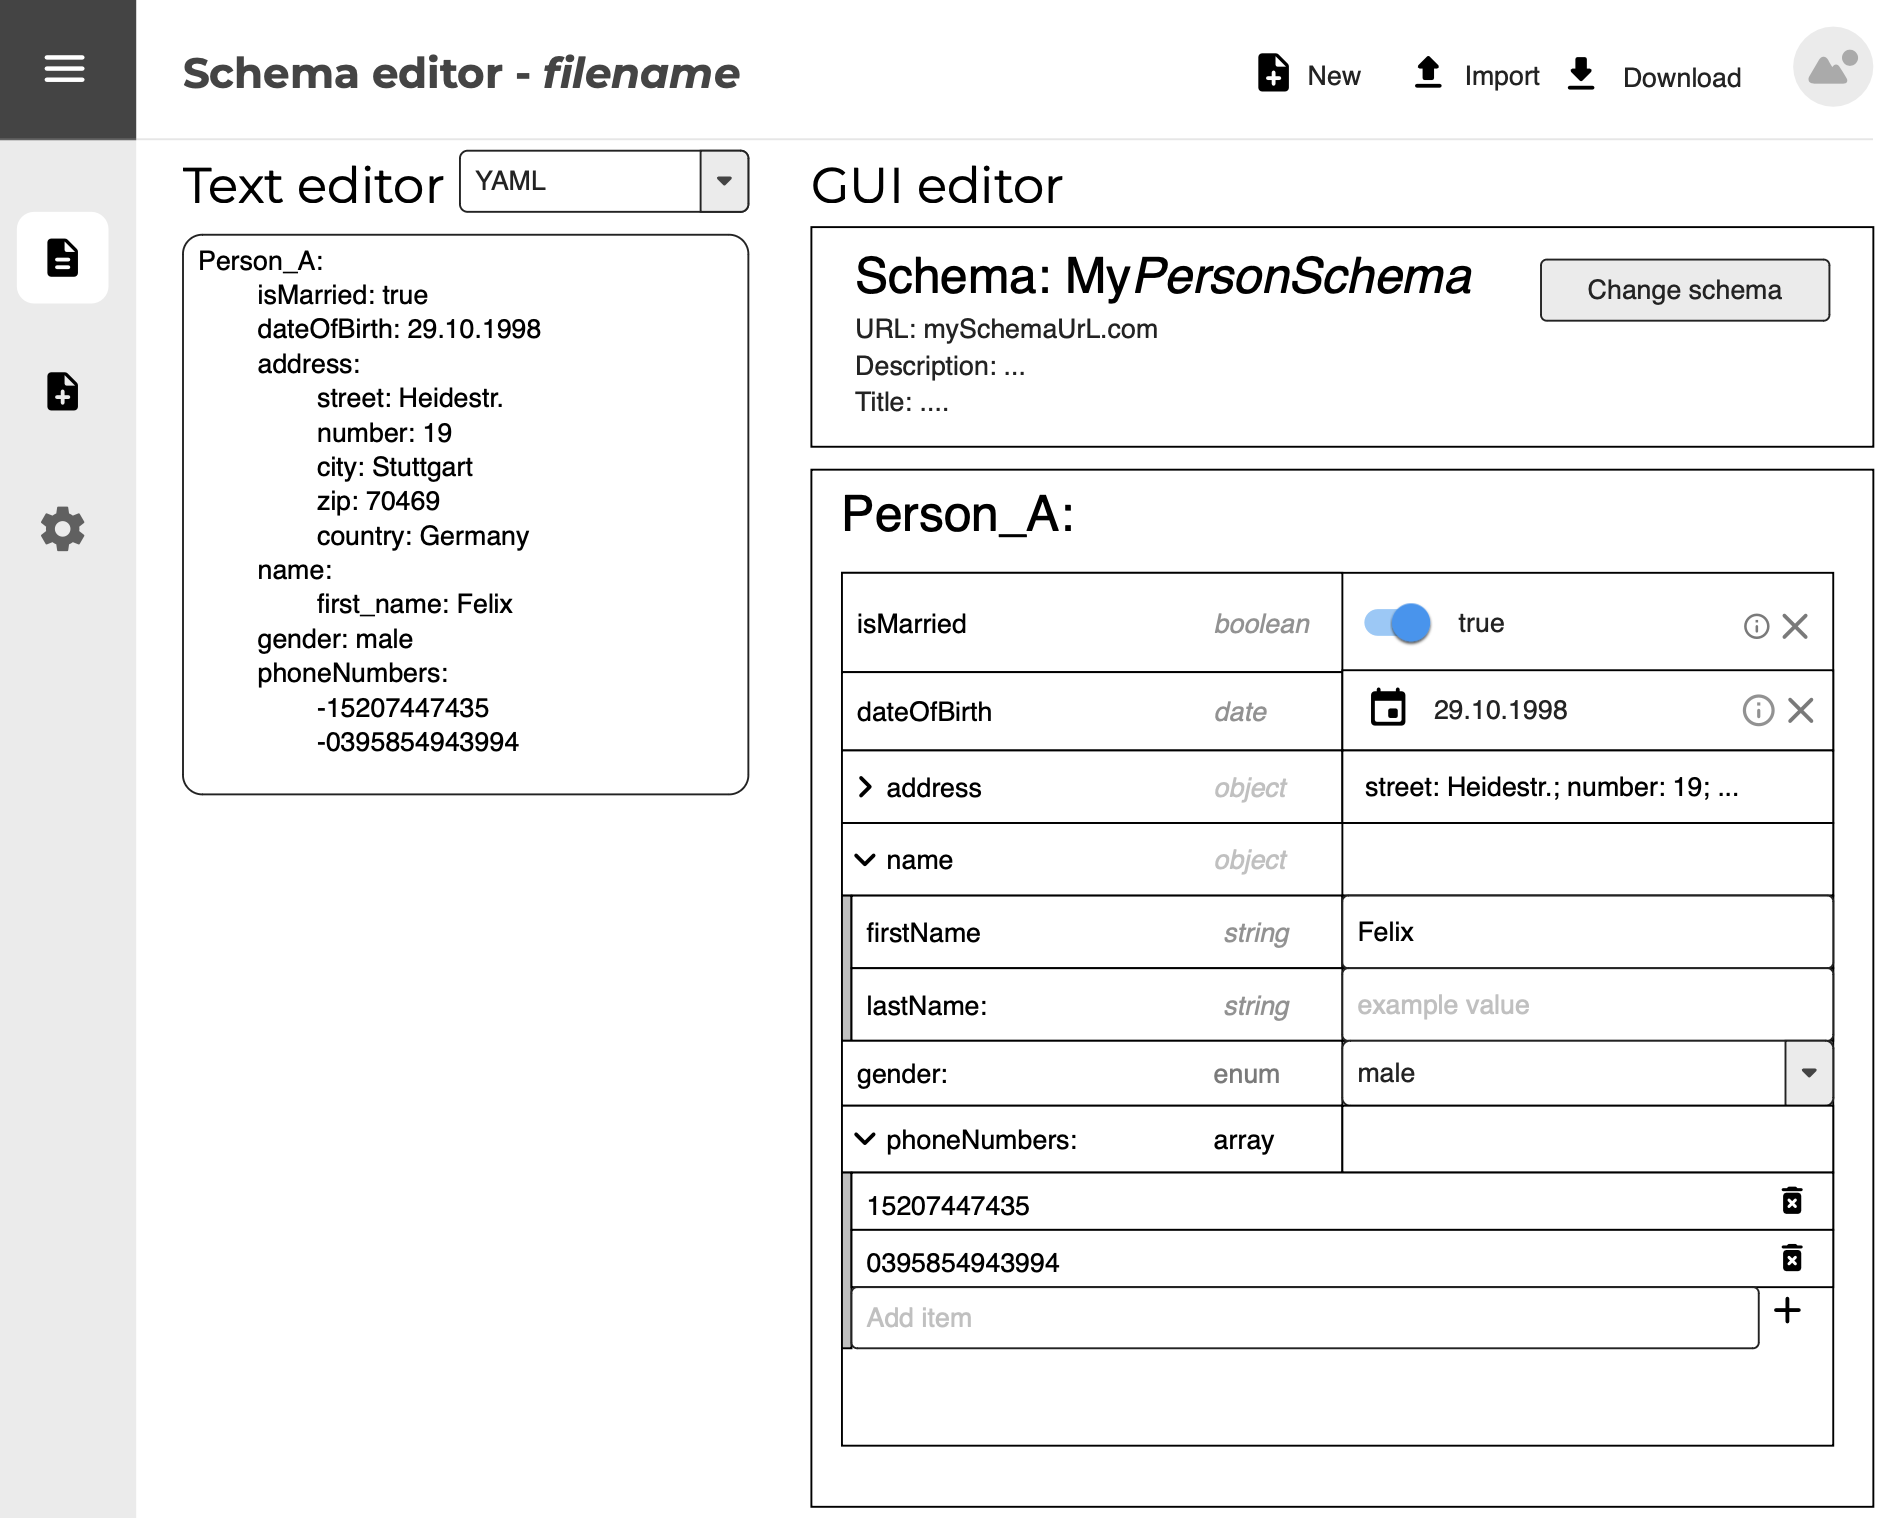
\includegraphics[width=\textwidth]{figures/mockup_gui_config}
    \caption{Sketch of the Tool before the implementation. File Editor view.}
    \label{mockup_gui_config}
\end{figure*}


\begin{figure*}[!thb]
    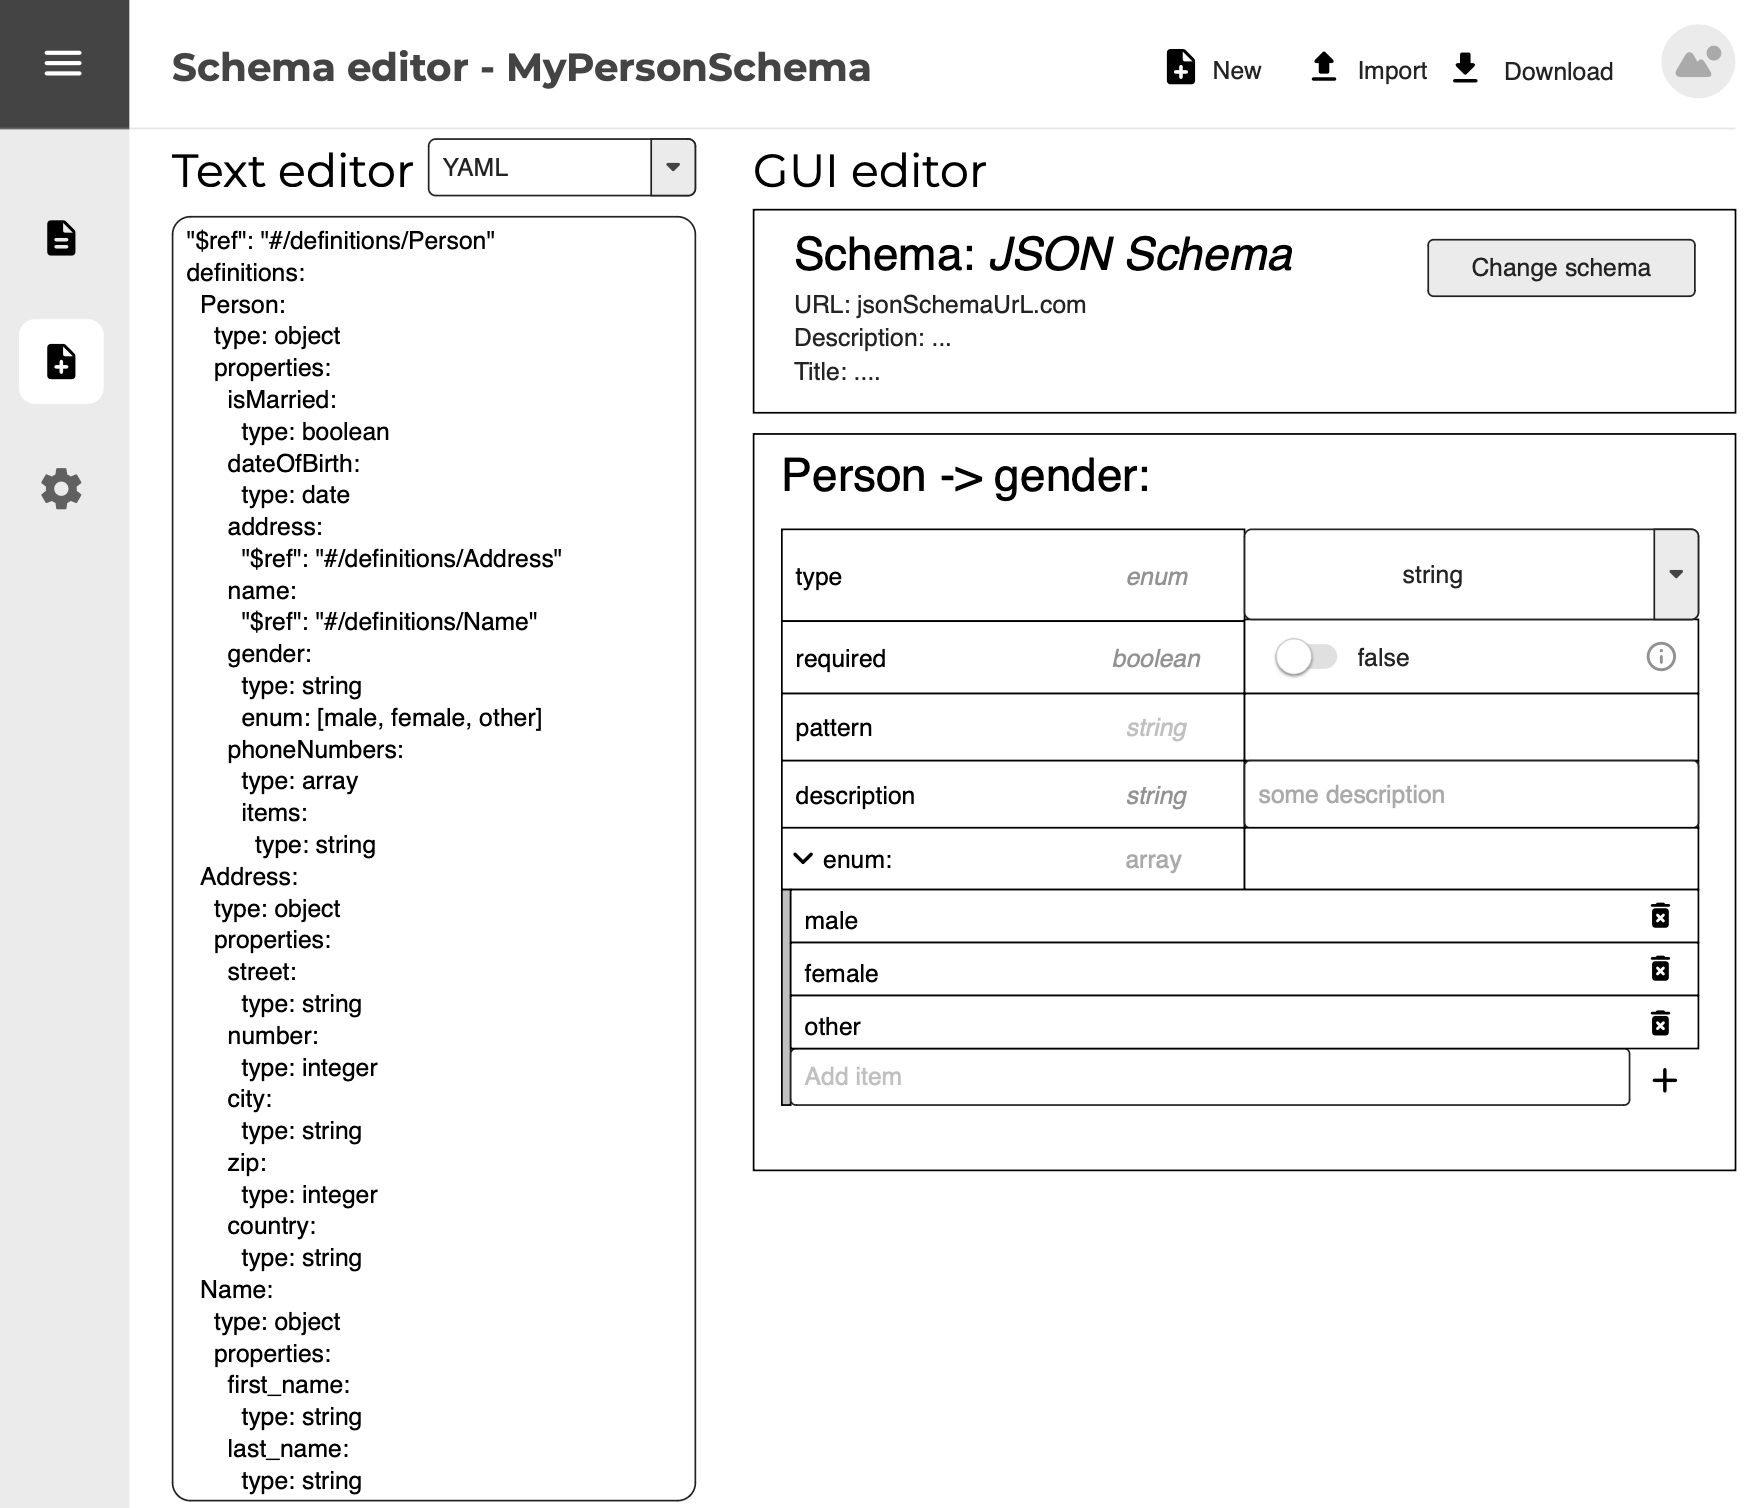
\includegraphics[width=\textwidth]{figures/mockup_gui_schema}
    \caption{Sketch of the Tool before the implementation. Schema Editor view.}
    \label{mockup_gui_schema}
\end{figure*}



\begin{figure*}[!htb]
    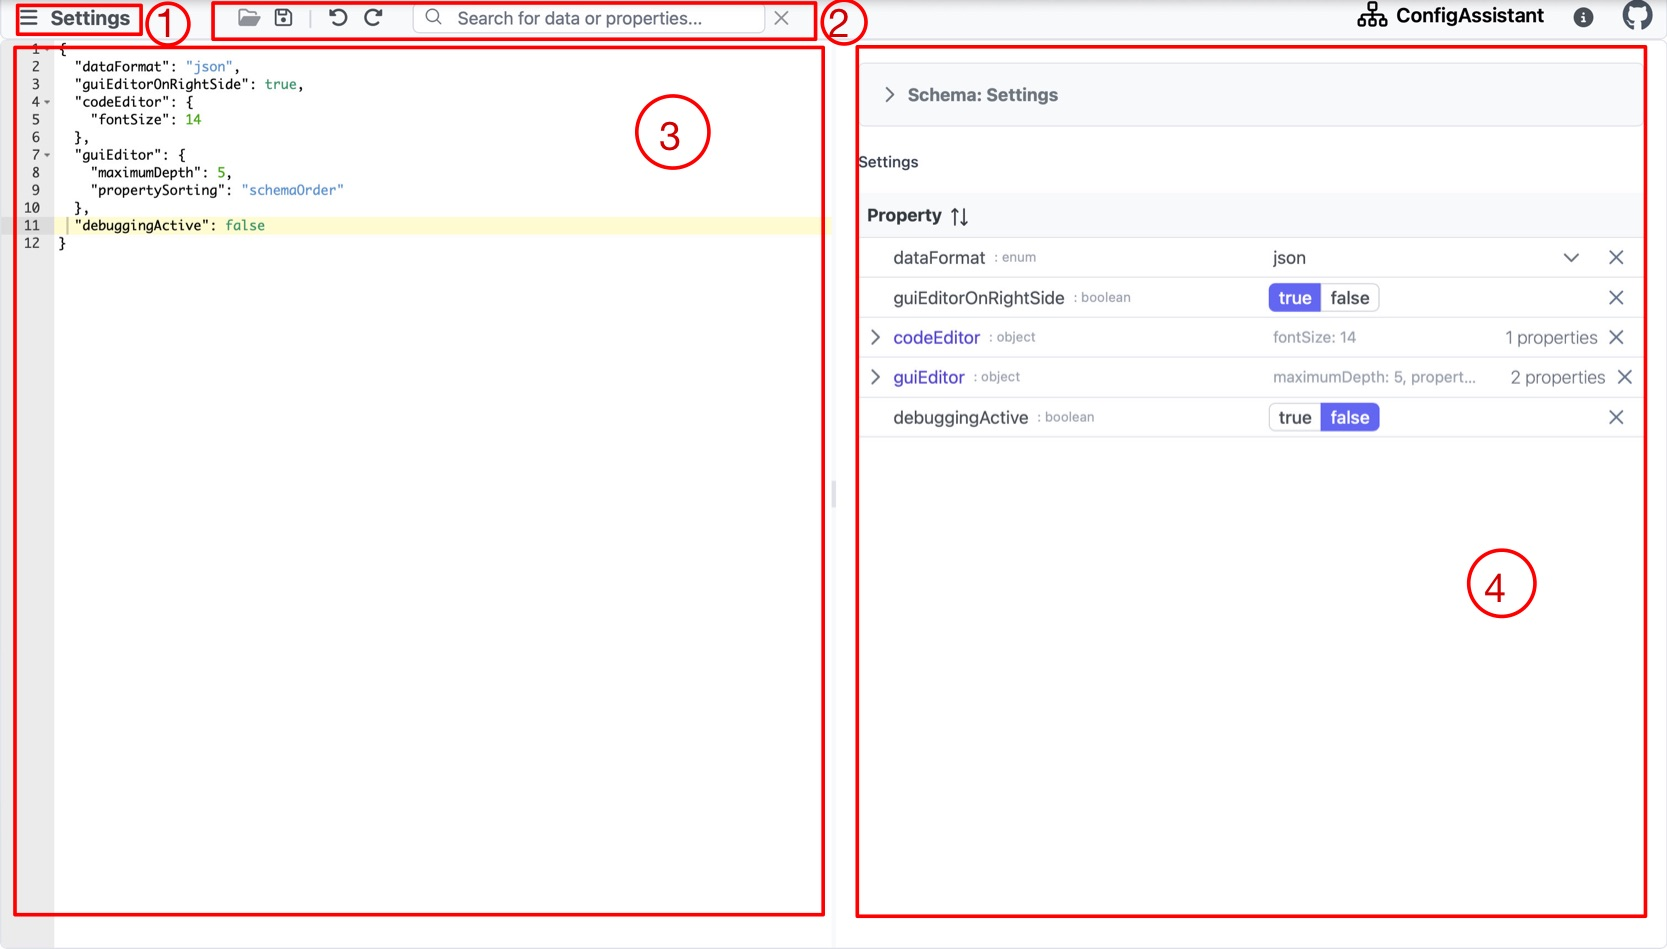
\includegraphics[width=\textwidth]{figures/settings}
    \caption{UI of Settings view}
    \label{fig:settings}
\end{figure*}



%\section{Implementation}\label{sec:appendix-implementation}
%\begin{table*}[!htb] % Use table* for wide tables
%    \caption{Libraries used in the implementation of our tool} %keyuri
%    \label{tab:libraries}
%    \centering
%    \begin{tabular}{ll}
%        \toprule
%        \textbf{Library} & \textbf{Purpose}     \\
%        \midrule
%        vue.js           & UI framework         \\
%        PrimeVue         & UI component library \\
%        Tailwind CSS     & CSS utility          \\
%        @fortawesome/fontawesome-svg-core & Font Awesome SVG icons. \\
%        ajv@8.12.0 & JSON schema validator for Node.js and browsers. \\
%        brace@0.11.1 & Browser-based code editor with syntax highlighting and code folding. \\
%        primeicons@6.0.1 & It is a popular UI component library for JavaServer Faces (JSF) applications. \\
%        \bottomrule
%    \end{tabular}
%\end{table*}


%\begin{table*}
%    \centering
%    \caption{Setting Parameters\label{tab:settings}}
%    \begin{tabular}{@{}p{0.3\linewidth}p{0.6\linewidth}@{}}
%        \toprule
%        \textbf{Parameter} & \textbf{\ Description} \\
%        \midrule
 %       Data Format & The data format used by the code editor. Currently YAML and JSON are supported. \\
 %       Code Editor Font Size & Size of the font in the code editor. \\
 %       Gui Editor On Right Side & By default, the GUI panel is located on the right side and the code panel on the left side. Using this option, their positions can be swapped. \\
%        GUI Editor Property Sorting & The order in which the properties in the GUI panel should appear:
%        \begin{itemize}
%            \item \textit{Schema Order}: Orders elements according to the order in the schema.
%            \item \textit{Priority Order}: Orders elements based on their priority (e.g. required properties first, deprecated %properties last).
%            \item \textit{Data Order }: Orders elements the same way as it is in the data.
%        \end{itemize} \\
%        GUI Editor Maximum Depth & Determines the maximum level of nesting or hierarchy displayed in the GUI editor. \\
%        Debugging Active & For debugging purposes, users can enable or disable the debugging panel as needed.  \\
%        \bottomrule
%    \end{tabular}
%\end{table*}


%\section{User Study}\label{sec:user-study}  % Minye
%\subsection{Interview Tasks}\label{subsec:tasks}
%This part is about the newest version of interview tasks we prepared to conduct our user study.\\
%\textbf{Remark:} Task 3 was added after the first user study and also some details in other tasks were modified.
%\subsubsection{Introduction}
%For these tasks you are presented a schema that you have not seen or worked with before.
%We have prepared a schema of a made-up simulation software in which self-driving cars are simulated.
%There is one self-driving car that has to navigate from a start point to an end point but there are also other vehicles and pedestrians simulated.
%For these tasks, the exact details are not important.
%
%\subsubsection{Task 1: Setup}
%\begin{enumerate}
%    \item Go to https://paulbredl.github.io/config-assistant/
%    \item Select the option ``Select a Schema'': ``Example schema'', then ``Autonomous Vehicle Schema".
%    \item Open the example configuration file we have sent to you. \\
%          The following tasks will assume this schema and this example file.
%\end{enumerate}
%
%\subsubsection{Task 2: Questions}
%\begin{enumerate}
%    \item What is the name of the simulation?
%    \item What is the weather in our simulated environment?
%    \item What is the total duration of the simulation?
%    \item Humidity is a subproperty of the Environment.
%    Would 150 be a valid value for Humidity?
%\end{enumerate}
%
%\subsubsection{Task 3: Modifying the configuration file}
%\begin{enumerate}
%    \item Change the name of the simulation to Sim\_Advanced05.
%    \item The VehicleType of the self-driving car is currently ``Level 3''.
%    Change it to the highest possible level.
%    \item The configuration file has validation errors, i.e., it is not valid according to the schema.
%    \\ Find out what the errors are.
%    Edit the file so it becomes a valid configuration.
%
%\end{enumerate}
%
%\subsubsection{Task 4: Modifying the schema}
%\begin{enumerate}
%    \item For many applications it is good practice or even required that a schema has a unique identifier, which usually is a URL.
%          \\Set the \$id field of this schema to : ``https://www.example.com/self-driving-vehicle''.
%    \item The simulation software will get a premium version in the next update, for which the user needs a license.
%          The license key should be stored in the configuration file.
%          Add a new property ``LicenseKey'' to the ``properties'' object.
%          It should be of the type ``string''.
%          The length of the key is at most 20 characters long.
%    Add a short exemplary description.
%    \item Go back to the file editor and verify that the new property ``LicenseKey'' is displayed and that the correct information is displayed when hovering over the property.
%\end{enumerate}





% Minye




\begin{table*}[!htbp] %keyuri
    \centering
    \caption{User Study 1 - Feedback and Solution}
    \label{table:user_study1}
    \begin{tabular}{p{0.45\linewidth}p{0.45\linewidth}}
        \toprule
         \thead{Feedback} & \thead{Solution} \\
        \midrule
        The property value should not be autocorrected if the user enters an incorrect value.
        Instead, an error message or another way should be used to inform the user that their input is incorrect.
        &
        Instead of autocorrecting values, we now provide more clear user feedback on incorrect values (red underline, error symbol). \\
        \midrule
        It would be good to have the ability to remove data entries with the GUI panel.
        &
        Implemented by adding a \textit{remove} button next to properties which have data and are not required. \\
        \midrule
        A search functionality to locate properties would be helpful, especially within nested levels.
        & Implemented in the toolbar.
        All findings are highlighted in the GUI panel. \\
        \midrule
        %& 4. The Schema editor GUI panel contains extensive metadata, but the code editor panel remains empty. & 4. bla bla bla \\
        %\midrule
        The GUI panel feels overwhelming to the user due to many variations in styling and color of the GUI elements.
        &
        We slightly reduced the number of different styling by no longer showing required properties in bold face and instead just show an asterisk next to it. \\
        \midrule
        The cursor should not have the clickable animation when hovering over non-clickable fields in the GUI editor.
        &
        Now we only show the clickable animation when hovering over clickable GUI components. \\
        \midrule
        In drop-down menus we do not need a button to clear the selection.
        &
        We disabled the option of clearing the selection. \\
        \midrule
        If the type of a property is ``any'', it should not be interpreted as the ``string'' type in the GUI panel.
        &
        We show a drop-down menu to the user, where they can select the type they want to use. \\
        \midrule
        Validation errors should not be highlighted via a warning symbol, but instead an error symbol.
        &
        We changed the warning symbol into an error symbol. \\
        \midrule
        After performing an undo or redo action, the cursor should jump to the corresponding location to reflect the changes made by the user.
        &
        Will be considered in future work. \\
        \bottomrule
    \end{tabular}
\end{table*}


\begin{table*} %keyuri

    \centering
    \caption{User Study 2 - Feedback and Solution}
    \label{table:user_study2}
    \begin{tabular}{p{0.45\linewidth}p{0.45\linewidth}}
        \toprule
        \thead{Feedback} & \thead{Solution} \\
        \midrule
        A graph-based view would be more intuitive for handling complex data structures.
        &
        Will be considered in future work. \\
        \midrule
        Providing immediate feedback to users when they enter incorrect ranges is essential to prevent them from inputting invalid values into the property.
        &
        We now highlight schema violations by a red error symbol in the GUI panel and underlining the property name in red.
        Additionally, the tooltip lists all schema violations of a property. \\
        \midrule
        Validation errors should also be reflected in the GUI panel, including for child properties.
        &
        See point above.
        Also, now the tooltip lists schema violations of child properties. \\
        \midrule
        When dealing with an array, the display name of array elements (index) should be improved.
        Currently, the tool only shows just the element index.
        &
        We replaced the numerical labels by a standard programming notation, which is \texttt{propertyName[0]}, \texttt{propertyName[1]}, \ldots
        \\
        \midrule
        The input field next to the \textit{Add Item} button is confusing.
        Both the input field and the button can be used to create a new item, which is redundant.
        &
        We removed the input field next to the button. \\
        \midrule
        It would be more consistent, if all user input in the GUI panel was within the right column of the table.
        That in some scenarios user input is needed within the left column (for names of new properties) feels inconsistent.
        &
        Because of the nature of JSON schema, we retained the property name within the left column.
        To make it clear to the user that the property name can be edited, we added an \textit{edit} icon next to it. \\
        \midrule
        The search function for locating specific properties lacks clarity at first glance.
        It should provide an immediate response and extend to nested levels, rather than merely highlighting the higher-level findings.
        &
        The search now provides a list of results, and upon clicking on a particular result, it jumps to that result in the code panel and GUI panel.
        In the GUI panel, if the element is nested, its parents will be automatically expanded. \\
        \bottomrule
    \end{tabular}

\end{table*}

\begin{table*} %keyuri
    \centering
    \caption{User Study 3 - Feedback and Solution} \label{table:user_study3}
    \begin{tabular}{p{0.45\linewidth}p{0.45\linewidth}}
        \toprule
        \thead{Feedback} & \thead{Solution} \\
        \midrule
        Working with the schema editor is difficult for me.
        It does not feel intuitive.
        &
        We made the schema editor more intuitive by creating our own simplified JSON schema meta schema.
        For example, advanced JSON schema features are separated from the simple ones.
        See section~\ref{subsec:schema-editor} \\
        \bottomrule

    \end{tabular}

\end{table*}

\begin{table*} %keyuri
    \centering
    \caption{User Study 4 - Feedback and Solution} \label{table:user_study4}
    \begin{tabular}{p{0.45\linewidth}p{0.45\linewidth}}
        \toprule
        \thead{Feedback} & \thead{Solution} \\
        \midrule
        Modifying or renaming a new property in the GUI panel does not appear to take effect when double-clicking on it.
        &
        Renaming properties in the GUI panel can now be done using the \textit{edit} button next to the property name. \\
        \midrule
        When creating a new property in the schema editor, its sub-schema has to be selected, such as \textit{string property} or \textit{boolean property}.
        Additionally, the type of the property has to be selected by the user too.
        Therefore, for example, when creating a new \textit{string property}, the user has to select that it is a string two times.
        It would be much more intuitive if the selection needs to be done only one time.
        & We completely overhauled our JSON schema meta schema.
        Now, when creating a new property, the user will have to select the type only once. \\
        \midrule
        A toggle button should be implemented to enable and disable the code panel and GUI panel.
        & Only having a GUI panel or only having a code panel restricts the user unnecessarily.
        The interplay of both panels is what makes this tool most effective.
         If the user does not want to use one of the panels, they can resize that panel to a very small size.  \\
        \midrule
        When working with a particular property in the GUI panel the opacity of the other properties should be decreased, visually highlighting the property that currently is in focus. & Will be considered in future work. \\
        \midrule
        Simplify the schema editor to make it easier to work with, for those who are not very familiar with JSON schema.
        &
        Has been done, see section~\ref{subsec:schema-editor}. \\
        \bottomrule

    \end{tabular}

\end{table*}

\begin{table*} %keyuri

    \centering
    \caption{User Study 5 - Feedback and Solution} \label{table:user_study5}
    \begin{tabular}{p{0.45\linewidth}p{0.45\linewidth}}
        \toprule
        \thead{Feedback} & \thead{Solution} \\
        \midrule
        The search button is not immediately evident, making it challenging for users to locate the search function. &
        Instead of showing the search bar only when clicking the search button, we now always show it. \\
        \bottomrule

    \end{tabular}

\end{table*}

\begin{table*} %keyuri
    \centering
    \caption{Use in Practice}\label{table:practical use and feedback}
    \begin{tabular}{p{0.1\linewidth}p{0.1\linewidth}p{0.1\linewidth}p{0.1\linewidth}p{0.25\linewidth}p{0.25\linewidth}}
        \toprule
        \textbf{User Study} & \textbf{Work Field/Profession} & \textbf{Would you use this tool yourself?} & \textbf{Potential Use case} & \textbf{Practical Use} & \textbf{Positive Feedback} \\
        \midrule
        1 & Professor & Yes & Configuring CI and simulations & Once the schema is loaded then one can start easily and after doing one time use, it will be easy to understand the 3 views. & "I think that the these two views always is very helpful." "And I, yeah, I think you also showed nice examples that you asked what is the Max value. Yeah, I wouldn't need to to jump back to the schema to find out what is the Max value right and now I can directly see what is the Max, what a levels do exist here and yeah." \\
        \midrule
        2 & Professor & Yes & Supervising projects in research data management & This tool will be recommended, and some project partners who require schema modification and extension will be invited. & "I think all complex uh schema, but otherwise I really like the tool and I think it's it's really, it's really very intuitive to work on the right hand side and it's good to have the overview on the left hand side in in a way I mean the combination of both views is is really helpful, really good." \\
        \midrule
        3 & Software Engineer & Yes & Research field in chemistry and biology & This tool is helpful to many people, such as scientists involved in data organization in the fields of chemistry and biology, rather than using Excel. It will be recommended to software engineers managing CI pipelines. It can also be used in the research field and promoted to partners for their use and sale of this tool. & "yeh, having clickable and intuitive way of showing structure in the tool looks pretty" "I understood the tool very well". "I am really impressed with this tool" \\
        \midrule
        4 & Professor & Yes & Chemistry and biology field &  Will be use this tool with own schema.
        It is useful even for those who have limited knowledge or understanding of schemas. & "yeh, looks nice, two windows is good idea and more easier and human readable". "Nested Properties are easier to find with this" \\
        \midrule
        5 & Student & Yes & Computer science field &  Computer science People as well non computer science People can use this tool only by loading JSON schema and do modification. & "There was pretty, like, positively surprised, like it was super easy to to kind of just navigate and it just made like parsing.
        JSON is always like a bit of a pain." "I can just like actually change things directly in in like a intuitive interface.So I yeah, it was pretty nice, I would say." \\
        \bottomrule
    \end{tabular}
\end{table*}
